% !TeX spellcheck = en_US

\chapter{Tasking Framework}
\section{Introduction}
Future unmanned space missions have a great demand on computing resources for the on-board data processing or for control algorithms. Also, future space missions are requested to achieve more and more challenging scientific goals \cite{PhdThesis}. Besides the pre-processing of scientific data to reduce the data amount for the downlink, it is also necessary to handle the control systems with optical sensors which come into play, for example for extra terrestrial navigation and landing systems \cite{ATON}. Space missions like the Rosetta mission or the landing of the Mars rover Curiosity were based on pre-defined timed command lists to control the landing \cite{TaskFr}. Because of this and the uncertainty of propulsion and parachute maneuver, the amount of different landing targets with low risks are considerably reduced \cite{TaskFr}. But the interesting areas of planetary research might also include risky landing areas and hence an autonomous control is needed for the spacecraft to control the trajectory and is is also needed to integrate hazard avoiding algorithms \cite{ATON}. However, these algorithms have a huge demand for computing power \cite{TaskFr}. 

In TET-1 satellite mission (Technology demonstrator) and \ac{bird} missions, the estimator and predictor modules were computed in a fixed order and fixed time in the control-cycle \cite{TETBIRD}. The timing was a combination of sensor latency and an additional gap time to satisfy the availability of data for computation and this led to a scant timing problem for the control torque computation due to over-estimated static safe-gap times \cite{TETBIRD}\cite{TETtoEUCROPIS}. During the \ac{leop}, a timing violation in another bus application resulted in changing the the order of inter-dependent computations and corrupted data, which further resulted in an unexpected \ac{aocs} state \cite{TETBIRD}. \cref{fig: Tasking} A) depicts such a situation and it can be observed that \texttt{ea = E(A)} is calculated before \texttt{eb = E(B)} 

On the other hand, the current on-board systems for the space environment do not provide the needed computing power \cite{TaskFr}. The space systems offer several controller boards on the spacecraft, most of them dedicated to only one subsystem and often twice for cold and hot redundancy. Such designs usually raise the power consumption and increase budgets like the mass, envelop and cost \cite{TaskFr}. Hence a concept, which allows sharing of computing resources based on predefined configurations for different flight phases and fault scenarios is necessary \cite{TaskFr}. The Tasking framework is an incarnation of the Inversion of Control design pattern which is popular practice in lightweight container frameworks \cite{InvOfCntrlurl}. 

A Tasking Framework is hence developed where the timing behavior is changed. Instead of starting computations at a predefined time in the computation cycle, a computation is started whenever the required information is available. All information are stored in messages distributed by channels and the channels initiate the computation when all the defined conditions for the computation are met \cite{TETBIRD}\cite{TETtoEUCROPIS}. The timing which can be achieved with Tasking Framework is as shown in \cref{fig: Tasking} B).    

\begin{figure}[h]
	\centering
	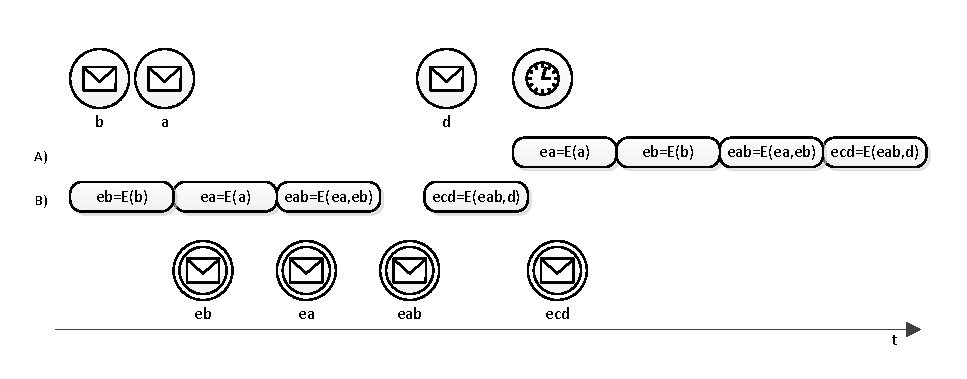
\includegraphics[width=0.8\textwidth]{TaskingFramework.pdf}
	\caption{Order and timing of computation tasks in BIRD and TET-1 vs order and timing of computation tasks in Eu:CROPIS}
	\source{\cite{TETtoEUCROPIS}}
	\label{fig: Tasking}
\end{figure}

\section{Usage of Tasking Framework}
The Tasking framework is based on C++ and provides some virtual base classes, which the application developer can overload to develop application specific computations. The Tasking Framework is designed to split the computations into small pieces, which are called tasks and they can be scheduled on the availability of the input data

For each task, a number of task inputs can be specified and each input can be associated with a task channel which provides the memory space and the synchronization for messages consumed by the task. In order to start a task, the task input needs to be configured with the expected number of pushes on the associated task channel and when the number of pushes on the task channel meets the expectation set, the respective task input is activated. When all the inputs of a particular task are activated, the task is automatically started by the scheduler of the Tasking Framework, provided a free computing core is available. If no computing core is available, then the task is queued for execution.

Any of the task inputs of a particular task can be marked as final and when such an input is activated, the respective task is started immediately by the scheduler irrespective of the activation states of the other task inputs. As a result, the task can push onto another channel, which can trigger the other task associated with this channel. This leads to a kind of behavior similar to petrinets, where the activation of the task input is a token and the task execution is a transition \cite{TaskFr}. The inputs associated to a task are reset when all its inputs are activated or when the respective activated input is marked as final. Such a reset operation on a task input sets the number of arrived data items on the associated task channel back to zero.

To specify timings in the Tasking framework, a special channel called 'event' is provided \cite{TaskFr}. An event is associated with a clock and the task input to which it is associated is notified on each clock tick. When the required number of notifications match the expected number which is already set, the attached task input is activated. Task event can be configured to work with absolute timing, i.e. the task input and in-turn the task is activated at fixed points in time, or the task event can be configured to work with a relative timing i.e, the task input and in-turn the task is activated at points in time relative to the execution time of the task.

To support mapping of tasks in a distributed system, task channels are associated with interfaces to read and write from and to networks and devices. These associations are set up by the configuration manager and are not visible to the application developer.

The current implementation of Tasking framework sits on top of Linux \ac{posix} library, composed by a real-time clock interface, signaling mechanism, memory access and the tasks scheduler. The Tasking framework can also run on \ac{rtems} and FreeRTOS using the outpost libraries which collectively provide a high level abstraction of the underlying operating system \cite{TaskFr}.

\section{Use cases for Tasking Framework}
In the project \ac{obc-ng} by \ac{dlr}, a decision is made to design the on-board computer systems as a combination of space qualified processing node, \ac{cots} processing nodes and network nodes \cite{TaskFr}. As an operating system for this project, an enhancement of \ac{rodos} is used \cite{TaskFr}\cite{OBC-NG}. The enhancement covers mainly the support for multi-core and reconfigurable distributed systems \cite{RODOS} and the core element which makes it possible is the Tasking Framework \cite{TaskFr}. The configuration manager used in OBC-NG holds predefined mappings of tasks and resources for different hardware configurations of computing resources and mission phases \cite{OBC-NG}. The communication infrastructure would be set up based on the mappings during the configuration phases of the system. 

The first usage of the Tasking framework was in the \ac{aton} project \cite{ATON}. The project was about the navigation system for a moon landing scenario. The project showed that the Tasking framework was a useful way for the parallelization of computations in an expected manner \cite{ATON}.

Another use-case of Tasking Framework is in the AOCS of \ac{eucropis} mission \cite{TETtoEUCROPIS}. Eu:CROPIS uses a porting of the Tasking framework from Linux to outpost libraries which collectively act as an operating system \ac{api} on top of RTEMS \cite{TETtoEUCROPIS}.

Tasking framework is also used in \ac{maius} which deals with activities to demonstrate Bose-Einstein condensation and atom interferometry with rubidium and potassium atoms on a sounding rocket \cite{TETtoEUCROPIS}\cite{MAIUS}.

\section{Use of Tasking Framework in this Master thesis}
Tasking framework is used as a computational model, as discussed in the previous chapter. The reasons for adopting are the following:

\begin{itemize}
\item The Tasking framework guarantees that the timing behavior of the system is deterministic and amenable to static analysis
\item The Tasking framework has been proven to be expressive enough to handle real-world application (refer previous section on use cases for Tasking framework)
\item Tasks do not interact with each other directly, but their communications are mediated by protected objects (task channels). These channels are shared resources equipped with a synchronization protocol in the form of priority based scheduling and \ac{fifo} scheduling for tasks with same priorities which uses these shared resources \cite{TaskFr}.  
\end{itemize}  

However, during the course of this Master thesis, certain short-comings of Tasking framework have been identified and they would be topics for discussion in the upcoming chapters

             



          